\newpage
%======================================================================
\section{Boundary Conditions}\label{chap:boundary-conditions}
%======================================================================





\begin{figure}[htbp]
	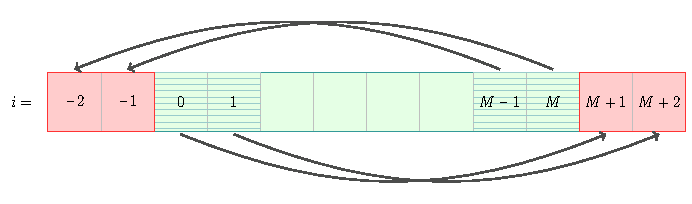
\includegraphics[width=\textwidth]{./figures/tikz/boundary_periodic.pdf}%
	\caption{\label{fig:boundary_periodic}
		Method to obtain periodic boundary conditions.
		The ghost cells are red, the arrows show what will be copied where.
	}
\end{figure}



\begin{figure}[htbp]
	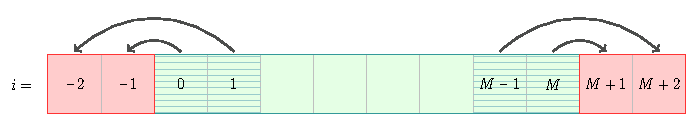
\includegraphics[width=\textwidth]{./figures/tikz/boundary_wall.pdf}%
	\caption{\label{fig:boundary_wall}
		Method to obtain wall boundary conditions.
		The ghost cells are red, the arrows show what will be copied where.
	}
\end{figure}



\begin{figure}[htbp]
	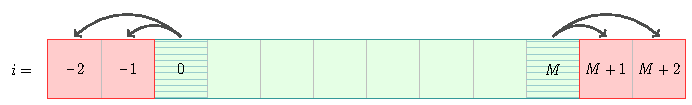
\includegraphics[width=\textwidth]{./figures/tikz/boundary_transmissive.pdf}%
	\caption{\label{fig:boundary_transmissive}
		Method to obtain transmissive boundary conditions.
		The ghost cells are red, the arrows show what will be copied where.
	}
\end{figure}



There are tricks how to obtain different kinds of boundary conditions.
In every case, we add additional cells (``\emph{ghost cells}'') in every dimension so we can simulate the desired behaviour.
How many cells you need to add depends on the methods (and mostly stencils) you use.
If you only take into account one neighbouring cell, then one ghost cell on every boundary suffices.
In figures \ref{fig:boundary_periodic}, \ref{fig:boundary_wall}, and \ref{fig:boundary_transmissive}, two ghost cells for a 1D grid are drawn.


Suppose we have 1D grid with $M$ cells and require 2 ghost cells each, which will have indices $-2$, $-1$, $M+1$, and $M+2$.
Then we can get:

\begin{itemize}
	\item \textbf{periodic boundary conditions:}
	
		what goes over the right edge, comes back in over the left edge, and vice versa.
		We achieve this behaviour by enforcing (fig. \ref{fig:boundary_periodic})
		\begin{align*}
			\U_{-2} &= \U_{M-1} \\
			\U_{-1} &= \U_{M}	\\
			\U_{M+1} &= \U_0 	\\
			\U_{M+2} &= \U_1 	\\
		\end{align*}
		
		
		
	\item \textbf{reflective boundary conditions:}
	
		pretend there is a wall at the boundary. 
		We achieve that by ``mirroring'' the cells next to the boundary (fig \ref{fig:boundary_wall}):

		\begin{align*}
			\U_{-2} &= \U_1		\\
			\U_{-1} &= \U_0		\\
			\U_{M+1} &= \U_{M}	\\
			\U_{M+2} &= \U_{M-1}\\
		\end{align*}
		
		However, every directional component (i.e. velocities/momentum) needs to have the negative value in the ghost cell compared to the real cell.
		
		This is valid for the Euler equations, but not for linear advection.
		In fact, having reflecting boundary conditions for constant linear advection doesn't really make sense.
	
	
	\item \textbf{transmissive boundary conditions}:
	
		Just let things flow out however they want. 
		We achieve this by copying the last boundary cell over and over again, such that it looks that the fluid appears to have that state infinitely, and there are no net fluxes to interfere with the hydrodynamics inside the actual grid (fig. \ref{fig:boundary_transmissive})
		
		
		\begin{align*}
			\U_{-2} &= \U_0		\\
			\U_{-1} &= \U_0		\\
			\U_{M+1} &= \U_{M}	\\
			\U_{M+2} &= \U_{M}	\\
		\end{align*}	
	
\end{itemize}



